\section{Integration von DevSecOps in den Software Development Lifecycle}

\subsection{Statische Code Analyse}

Statische Code Analyse ist ein entscheidender Schritt im DevSecOps-Prozess, um die Sicherheit und Qualität des Codes bereits frühzeitig im Entwicklungsprozess zu gewährleisten. Durch den Einsatz von Tools zur statischen Code Analyse können potenzielle Sicherheitslücken, Code-Smells und andere Qualitätsprobleme automatisch erkannt werden. In diesem Kapitel werden wir die Integration von statischer Code Analyse in eine CI/CD-Pipeline anhand von SonarQube und GitHub Actions demonstrieren.

\subsubsection{Übersicht der Tools zur statischen Code Analyse}

Es gibt eine Vielzahl von Tools, die zur statischen Code Analyse eingesetzt werden können. Die folgende Tabelle gibt eine Übersicht über einige gängige Tools:

\begin{table}[h!]
\centering
\begin{tabular}{|l|l|l|l|}
\hline
\textbf{Tool} & \textbf{Programmiersprachen} & \textbf{Lizenz} & \textbf{Besonderheiten} \\ \hline
SonarQube & Mehrere & Open Source & Umfangreiche Analyse, Integration in CI/CD \\ \hline
ESLint & JavaScript, TypeScript & Open Source & Speziell für JavaScript, konfigurierbar \\ \hline
Checkmarx & Mehrere & Proprietär & Fokus auf Sicherheit \\ \hline
PMD & Java, Apex & Open Source & Regelbasierte Analyse \\ \hline
Bandit & Python & Open Source & Sicherheitsanalyse für Python \\ \hline
\end{tabular}
\caption{Übersicht von Tools zur statischen Code Analyse}
\label{tab:static_code_analysis_tools}
\end{table}

\subsubsection{Integration von SonarQube in die CI/CD-Pipeline}

SonarQube ist ein weit verbreitetes Tool zur statischen Code Analyse, das eine nahtlose Integration in CI/CD-Pipelines unterstützt. Im Folgenden wird gezeigt, wie SonarQube mit GitHub Actions integriert werden kann, um eine automatisierte Analyse des Codes durchzuführen.

\paragraph{Einrichtung von SonarQube}

1. Installation und Konfiguration von SonarQube.
2. Erstellung eines neuen Projekts in SonarQube.
3. Generierung eines Tokens für die Authentifizierung in GitHub Actions.

\paragraph{Konfiguration der GitHub Actions Workflow-Datei}

Erstellen Sie im Wurzelverzeichnis Ihres Repositories eine Datei namens \texttt{.github/workflows/sonarqube.yml} mit folgendem Inhalt:

\begin{verbatim}
name: SonarQube Analysis

on:
  push:
    branches:
      - main
      - develop
  pull_request:
    branches:
      - main
      - develop

jobs:
  sonarQube:
    runs-on: ubuntu-latest

    steps:
    - name: Check out repository
      uses: actions/checkout@v2

    - name: Set up JDK 11
      uses: actions/setup-java@v1
      with:
        java-version: '11'

    - name: Cache SonarQube packages
      uses: actions/cache@v2
      with:
        path: ~/.sonar/cache
        key: ${{ runner.os }}-sonar-cache
        restore-keys: ${{ runner.os }}-sonar-cache

    - name: Install dependencies
      run: ./gradlew build -x test

    - name: Run SonarQube analysis
      env:
        SONAR_TOKEN: ${{ secrets.SONAR_TOKEN }}
      run: ./gradlew sonarqube -Dsonar.projectKey=my_project_key -Dsonar.host.url=https://sonarqube.mycompany.com -Dsonar.login=${{ secrets.SONAR_TOKEN }}
\end{verbatim}

\paragraph{Branch-Regeln und Merge-Policies}

Um sicherzustellen, dass nur Code, der den definierten Sicherheitsstandards entspricht, in die Haupt-Branches integriert wird, können Branch-Regeln und Merge-Policies in GitHub konfiguriert werden. Hierbei wird beispielsweise das Mergen von Branches blockiert, die den OWASP-Standards in SonarQube nicht entsprechen.

\begin{itemize}
    \item Gehe zu den Einstellungen des Repositories auf GitHub.
    \item Wähle \textit{Branches} und dann \textit{Branch protection rules}.
    \item Erstelle eine neue Regel für den \textit{main} und \textit{develop} Branch.
    \item Aktiviere die Option \textit{Require status checks to pass before merging} und füge den SonarQube-Status hinzu.
\end{itemize}

\subsection{Beispielkonfiguration und Demonstration}

\subsubsection{Erstellung und Verwendung des GitFlow-Modells}

Das GitFlow-Modell ist ein weit verbreitetes Workflow-Modell, das die Arbeit mit Feature-Branches und Release-Branches strukturiert. Es wird folgendermaßen implementiert:

\begin{itemize}
    \item \textbf{main}: Enthält den Produktionscode.
    \item \textbf{develop}: Basis für neue Features.
    \item \textbf{feature-branches}: Abgeleitet von \textit{develop}, für die Entwicklung neuer Features.
    \item \textbf{release-branches}: Vorbereitung für neue Releases.
    \item \textbf{hotfix-branches}: Dringende Korrekturen auf dem \textit{main}-Branch.
\end{itemize}

\paragraph{Workflow-Illustration}

\begin{figure}[h!]
\centering
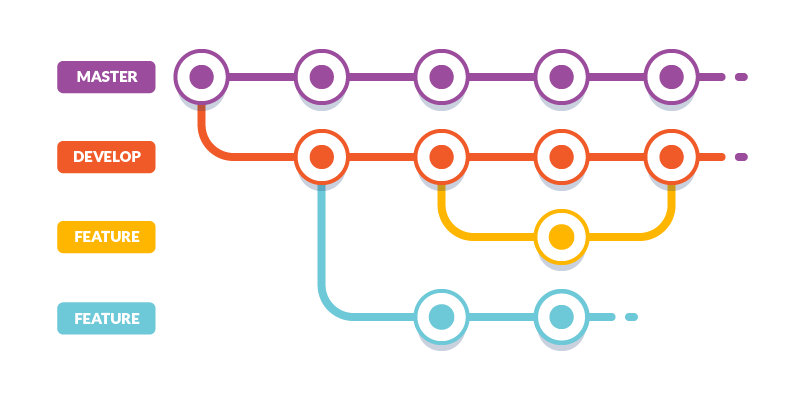
\includegraphics[width=\textwidth]{gitflow_workflow.png}
\caption{Illustration des GitFlow-Modells}
\label{fig:gitflow}
\end{figure}

\paragraph{Beispielhafte Umsetzung in GitHub}

\begin{enumerate}
    \item Forke das Repository und erstelle einen neuen Branch: \texttt{git checkout -b feature/new-feature develop}
    \item Implementiere das neue Feature und pushe die Änderungen: \texttt{git push origin feature/new-feature}
    \item Öffne einen Pull Request von \texttt{feature/new-feature} nach \texttt{develop}.
    \item Die CI/CD-Pipeline führt die statische Code Analyse mit SonarQube durch.
    \item Bestehen alle Checks, kann der Branch gemerged werden.
\end{enumerate}

\paragraph{Screenshots und Ergebnisinterpretation}

Fügen Sie hier passende Screenshots ein, die die Ergebnisse der SonarQube-Analyse und den Workflow der GitHub Actions demonstrieren.

\begin{figure}[h!]
\centering
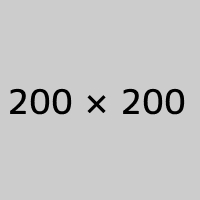
\includegraphics[width=\textwidth]{sonarqube_results.png}
\caption{Ergebnisse der SonarQube-Analyse}
\label{fig:sonarqube_results}
\end{figure}

\subsubsection{Schlussfolgerungen und Best Practices}

Die Integration von statischer Code Analyse in den CI/CD-Prozess verbessert nicht nur die Codequalität, sondern trägt auch zur Erhöhung der Sicherheit bei. Durch den Einsatz von Tools wie SonarQube in Kombination mit GitHub Actions und strikten Branch-Regeln können potenzielle Schwachstellen frühzeitig erkannt und behoben werden.


\end{document}
